\begin{frame}
\frametitle{About This Work...}

\emph{Leveraging Spatio-Temporal Redundancy for RFID Data Cleansing}.~\cite{chen2010leveraging} \\
H.~Chen, W-S.~Ku, H.~W and M-T.~S.\\~\\

\begin{itemize}
  \item Published at \emph{SIGMOD' 2010}.
  \item Proposed a Bayesian inference based approach for cleaning RFID raw data.
  \item Designed an $n$-state detection model to capture the likelihood.
  \item Devised a Metropolis-Hastings sampler with Constraints (MH-C) to sample from the posterior.
\end{itemize}

\end{frame}

%------------------------------------------------

\begin{frame}
\frametitle{Motivation}

To take full advantage of:

\begin{itemize}
  \item duplicate readings (by multiple readers simultaneously or by a single reader over a period of time) of the same object are very common.
  \item prior knowledge about the readers and the environment (e.g., prior data distribution, false negative rates of readers) may help improve data quality and remove data anomalies.
  \item given constraints in target applications (e.g., the number of objects in a same location cannot exceed a given value).
\end{itemize}

\end{frame}

%------------------------------------------------

\begin{frame}
\frametitle{Data Redundancy: Spatial Redundancy\cite{jeffery2006adaptive, rao2006deferred}}

\fsize{\textrm{The challenge is how to take advantage of redundancy while avoiding its undesirable effect in data cleansing.}}

\vspace{-10pt}
\begin{columns}[c]

  \column{0.5\textwidth}
  \begin{figure}[tb]
    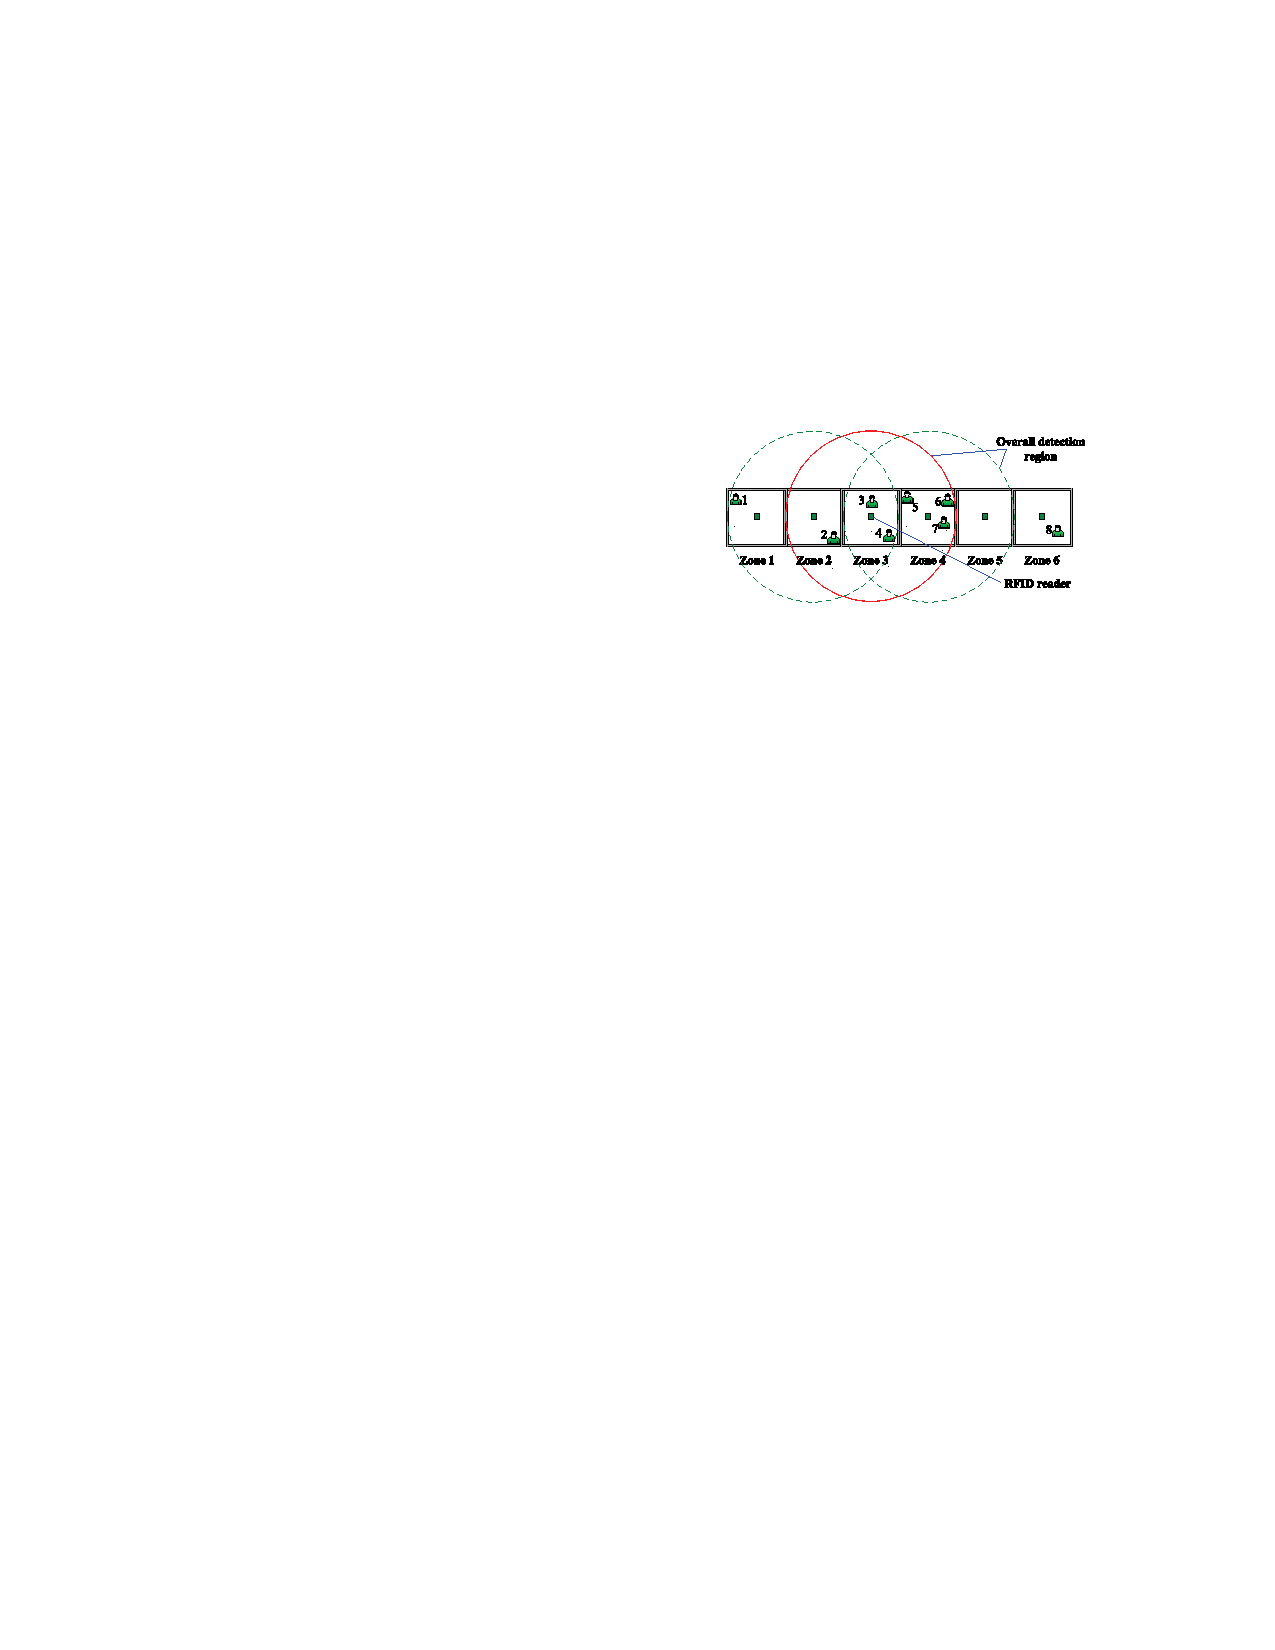
\includegraphics[width=\columnwidth]{figures/3-1/3-1-2.pdf}
  \end{figure}

  \begin{example}
    \ssize{
    \textrm{
    the target area is divided into 6 zones, an RFID reader is located in the center of each zone. Spatial overlap of readers' detection regions leads to duplicate readings, i.e., an object is in the detection regions of multiple readers.
    }}
  \end{example}

  \column{0.5\textwidth}
  \begin{figure}[tb]
    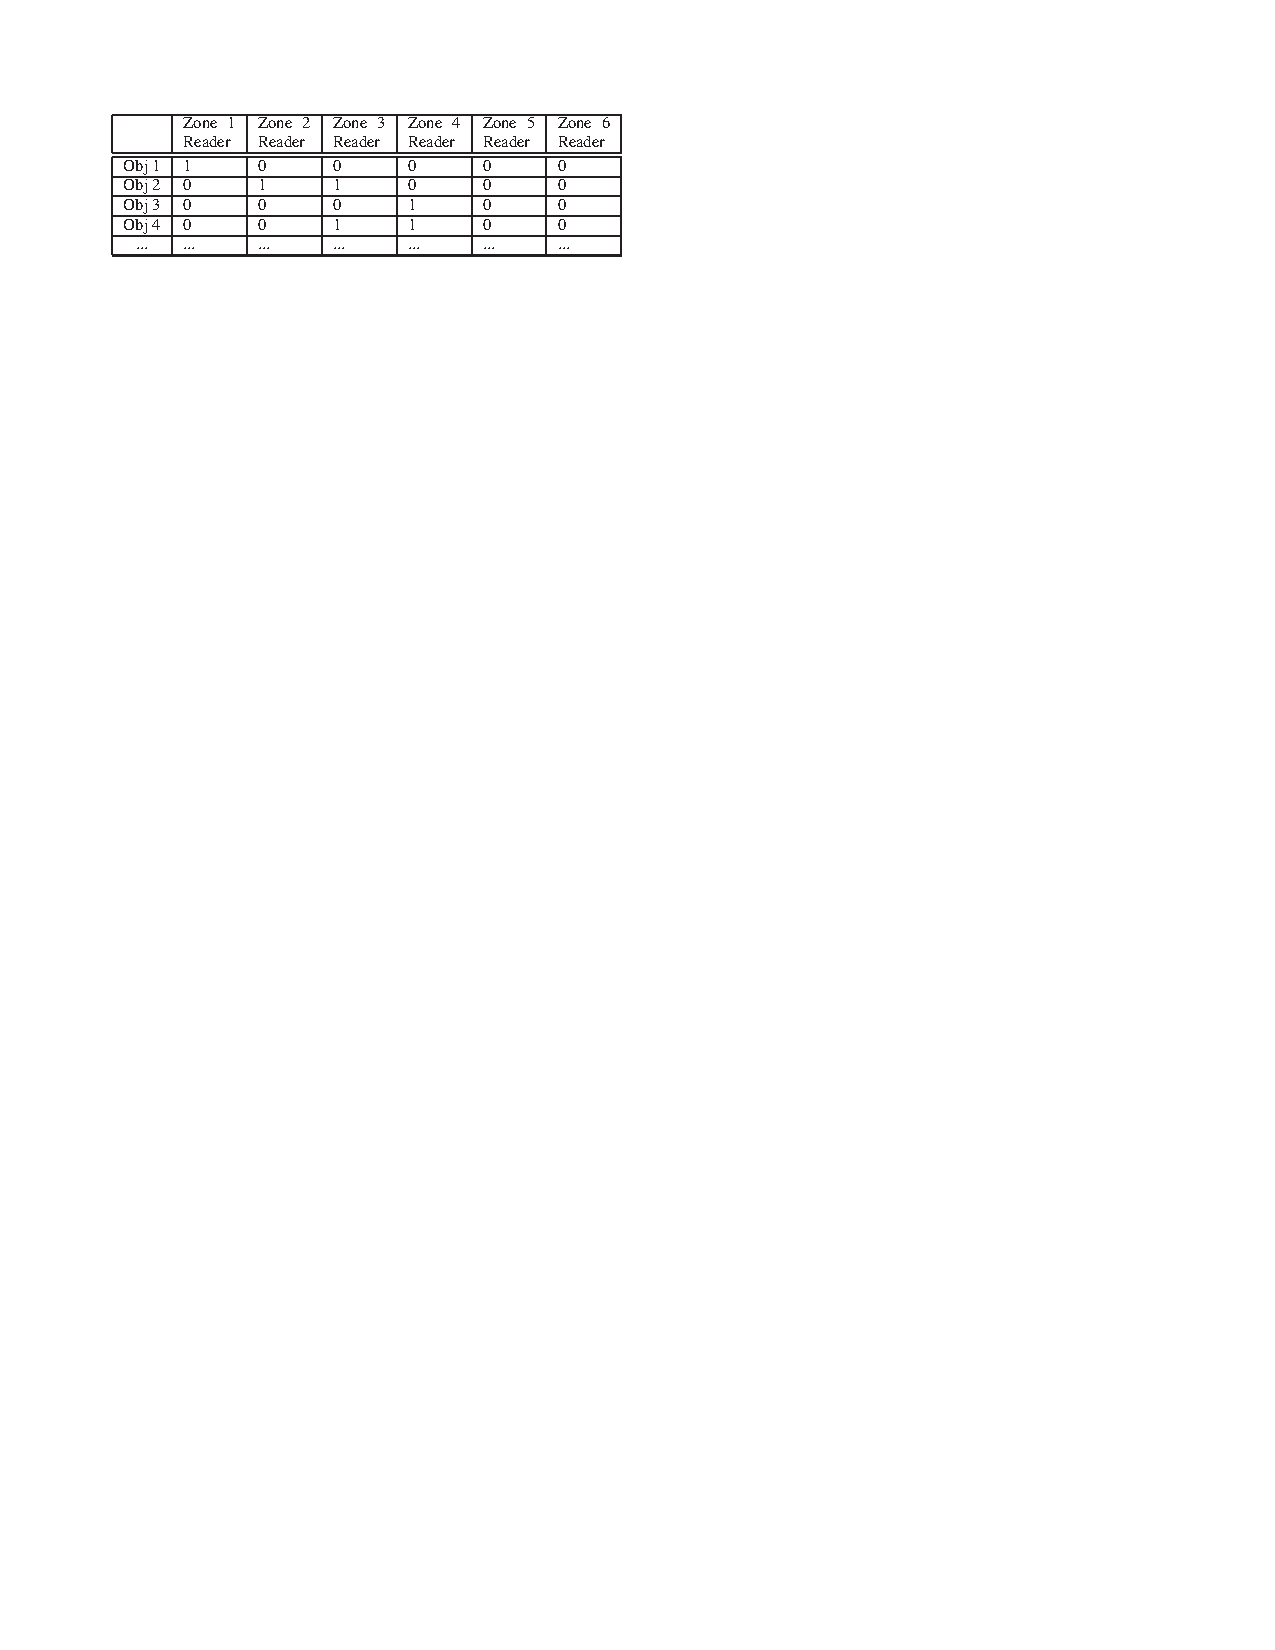
\includegraphics[width=\columnwidth]{figures/3-1/3-1-1.pdf}
  \end{figure}

  \ssize{
  The above table shows two effects of redundancy:
  \begin{enumerate}
    \item Object 2 is detected by both readers in Zone 2 and 3, at least one of the readings belongs to spatial redundancy.
    \item Object 3 is detected in Zone 4 only, however, it does not necessarily mean that the Object 3 is in Zone 4 for sure.
  \end{enumerate}
  }

\end{columns}

\end{frame}

%------------------------------------------------

\begin{frame}
\frametitle{Data Redundancy: Temporal Redundancy}

Many applications monitor the target area using a \emph{mobile reader} instead of employing multiple \emph{stationary readers}.\\~\\

Because the exact location of the mobile reader is always changing, the detection regions at different time points may overlap.\\~\\

\textbf{The temporal redundancy problem can be reduced to the spatial redundancy problem:} by treating the same reader at different time points as different readers.

\end{frame}

%------------------------------------------------

\begin{frame}
\frametitle{Prior Knowledge}

As false negatives and false positives abound in raw RFID readings, in order to recover the true information, the data cleansing system should take prior knowledge into account.\\~\\

For example, the detection areas of readers in Zone 2 and 3 have significant overlapping, the positioning of the reader in Zone 4 makes it more likely to detect objects in Zone 3 than objects in Zone 5, or the reader in Zone 3 has high false negative rate.

\end{frame}

%------------------------------------------------

\begin{frame}
\frametitle{Constraints}

\emph{Environmental constraints} can be utilized to improved data cleansing.\\~\\

For example, the maximal capacity of each zone (the number of objects that can reside the same zone) is a constraint.\\~\\

In addition to these physical constraints, information obtained from other channels can be translated into constraints. E.g., if an extra source indicates that two certain objects are in the same zone, it may help cleanse the data of there two.

\end{frame}

%------------------------------------------------

\begin{frame}
\frametitle{Overview of the Approach}

\begin{enumerate}
  \item By using Bayesian inference, it derives a universal framework of computing the posterior probabilities (of the location of each object).
  \item Based on the physical characteristic of RFID readers, it proposes an $n$-state detection model to capture likelihoods.
  \item It devised MH-C, an improved \emph{Metropolis-Hastings} sampler, to sample from the posterior while taking the environmental constraints into consideration.
\end{enumerate}

\end{frame}

%------------------------------------------------

\begin{frame}
\frametitle{Notations}

\begin{figure}[tb]
  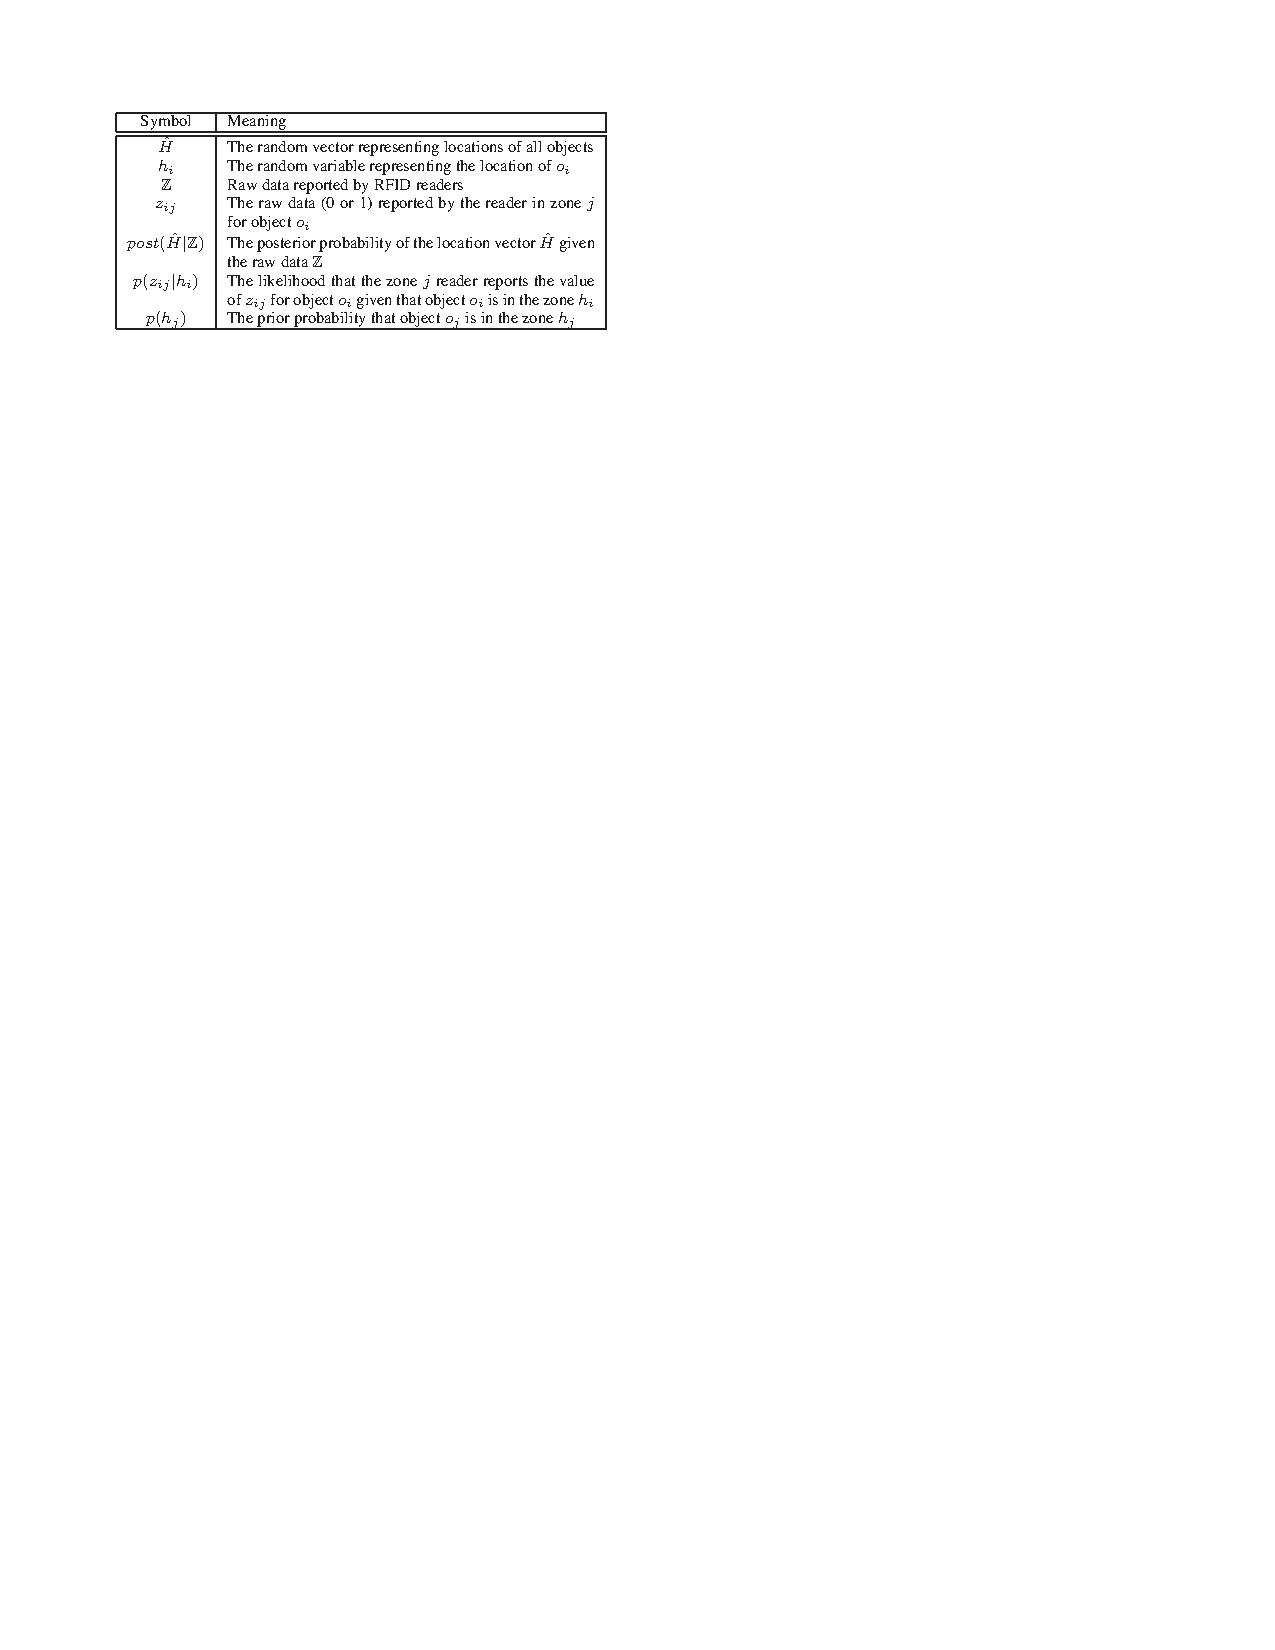
\includegraphics[width=\columnwidth]{figures/3-1/3-1-3.pdf}
\end{figure}

\end{frame}

%------------------------------------------------

\begin{frame}
\frametitle{A Bayesian Interface Base Approach}

\conceptbf{Bayesian Interface} estimates the probability of a hypothesis $(x)$ based on observations $(y)$, showing that posterior is proportional to the multiplication of likelihood and prior, i.e., $p(x|y) \propto p(y|x)p(x)$.\\~\\\pause

Suppose there're $m$ zones (each with a reader mounted in the center) and $n$ objects. For each object $o_i$, its location is represented by a random variable $h_i$. A possible distribution of $n$ objects in $m$ zones can be denoted as an instance of the random vector:\pause
\begin{equation}
  \hat{H} = \{ h_1, h_2, ..., h_n \}
\end{equation}
\pause

where $h_i$ represents the zone ID where object $o_i$ is in. E.g., $h_1 = 2$ denotes that object $o_1$ is in zone 2 in the current instance.

\end{frame}

%------------------------------------------------

\begin{frame}
\frametitle{A Bayesian Interface Base Approach}

For the reader in zone $j$, the raw data (0 or 1) it receives from the RFID tag of objects $o_i$ is denoted as $z_{ij}$. Thr \emph{raw data matrix} for each complete scan from $m$ readers can then be represented as an $n \times m$ matrix $\mathbb{Z} = [z_{ij}]$. \\~\\ \pause

Using the \conceptbf{Bayesian theorem}, where $post(\hat{H}|\mathbb{Z})$ denotes the posterior probability of location vector $\hat{H}$ given the raw data matrix $\mathbb{Z}$. The hypothesis should satisfy all constraints: \pause
\begin{equation}
  \begin{split}
  post(\hat{H}|\mathbb{Z}) = 0 & :\hat{H} \textrm{ is not valid} \\
  post(\hat{H}|\mathbb{Z}) > 0 & :\hat{H} \textrm{ is valid} \\
  post(\hat{H_1}|\mathbb{Z}) > post(\hat{H_2}|\mathbb{Z}) & :\hat{H_1} \textrm{ is more likely than } \hat{H_2}
  \end{split}
\end{equation}

\end{frame}

%------------------------------------------------

\begin{frame}
\frametitle{Computation on Posterior of Each Sample}

\begin{equation*}
  \begin{split}
  post(\hat{H}|\mathbb{Z}) & = post(h_1, h_2, ..., h_n | \begin{bmatrix}
 z_{11} & \cdots & z_{1m} \\
 \vdots & \ddots & \vdots \\
 z_{n1} & \cdots & z_{nm}
\end{bmatrix}) \\
 & \propto p(\begin{bmatrix}
z_{11} & \cdots & z_{1m} \\
\vdots & \ddots & \vdots \\
z_{n1} & \cdots & z_{nm}
\end{bmatrix} | h_1, h_2, ..., h_n) \cdot p(h_1, h_2, ..., h_n)
  \end{split}
\end{equation*}
\pause

\emph{Assume that each reader detects the tags of different objects independently.} \pause

\begin{equation*}
  post(\hat{H}|\mathbb{Z}) \propto \prod_{i}p(z_{i1},z_{i2},...z_{im} | h_1, h_2, ..., h_n) \cdot p(h_1, h_2, ..., h_n)
\end{equation*}


\end{frame}

%------------------------------------------------

\begin{frame}
\frametitle{Computation on Posterior of Each Sample}

\begin{equation*}
  post(\hat{H}|\mathbb{Z}) \propto \prod_{i}p(z_{i1},z_{i2},...z_{im} | h_1, h_2, ..., h_n) \cdot p(h_1, h_2, ..., h_n)
\end{equation*}
\pause

\emph{Assume that each each reader's detection of the same object does not depend on that of other objects, also, the prior distribution of each object does not depend on that of other objects.} \pause

\begin{equation*}
  \begin{split}
  post(\hat{H}|\mathbb{Z}) & \propto \prod_{i} p(z_{i1} | h_i) \cdot p(z_{i2} | h_i) \cdot ... \cdot p(z_{im} | h_i) \cdot \prod_{j} p(h_j) \\
  & = \alpha \cdot \prod_{i} p(z_{i1} | h_i) \cdot p(z_{i2} | h_i) \cdot ... \cdot p(z_{im} | h_i) \cdot \prod_{j} p(h_j)
  \end{split}
\end{equation*}
\pause

\end{frame}

%------------------------------------------------

\begin{frame}
\frametitle{The Goal}

Based on the equation, given the raw reading $\mathbb{Z}$ and a hypothesis $\hat{H}$ (the location of each object), one can derive the probability of the hypothesis.\\~\\

However, finding just one valid hypothesis will provide nothing more than a biased answer to queries against the uncertain data.\\~\\

It is \emph{unrealistic} to find all valid hypotheses, thus, the \conceptbf{goal} is to create a large sample set of valid hypotheses, each associated with a weight computed by the posterior computation equation.\\~\\

The sample set of valid hypotheses as a whole enables answering queries with high credibility.

\end{frame}

%------------------------------------------------

\begin{frame}
\frametitle{The Obstacles}

\begin{itemize}
  \item A prerequisite for effective hypothesis sampling is to be able to compute the posterior probability of each hypothesis precisely.\\~\\
  \item The hypothesis space is high dimensional, and the posterior probability is difficult to sample from.\\~\\
  \item It needs to incorporate constraint management in sampling.
\end{itemize}

\end{frame}

%------------------------------------------------

\begin{frame}
\frametitle{RFID Reader Detection Model: A simplified 2-State}

\begin{figure}[tb]
  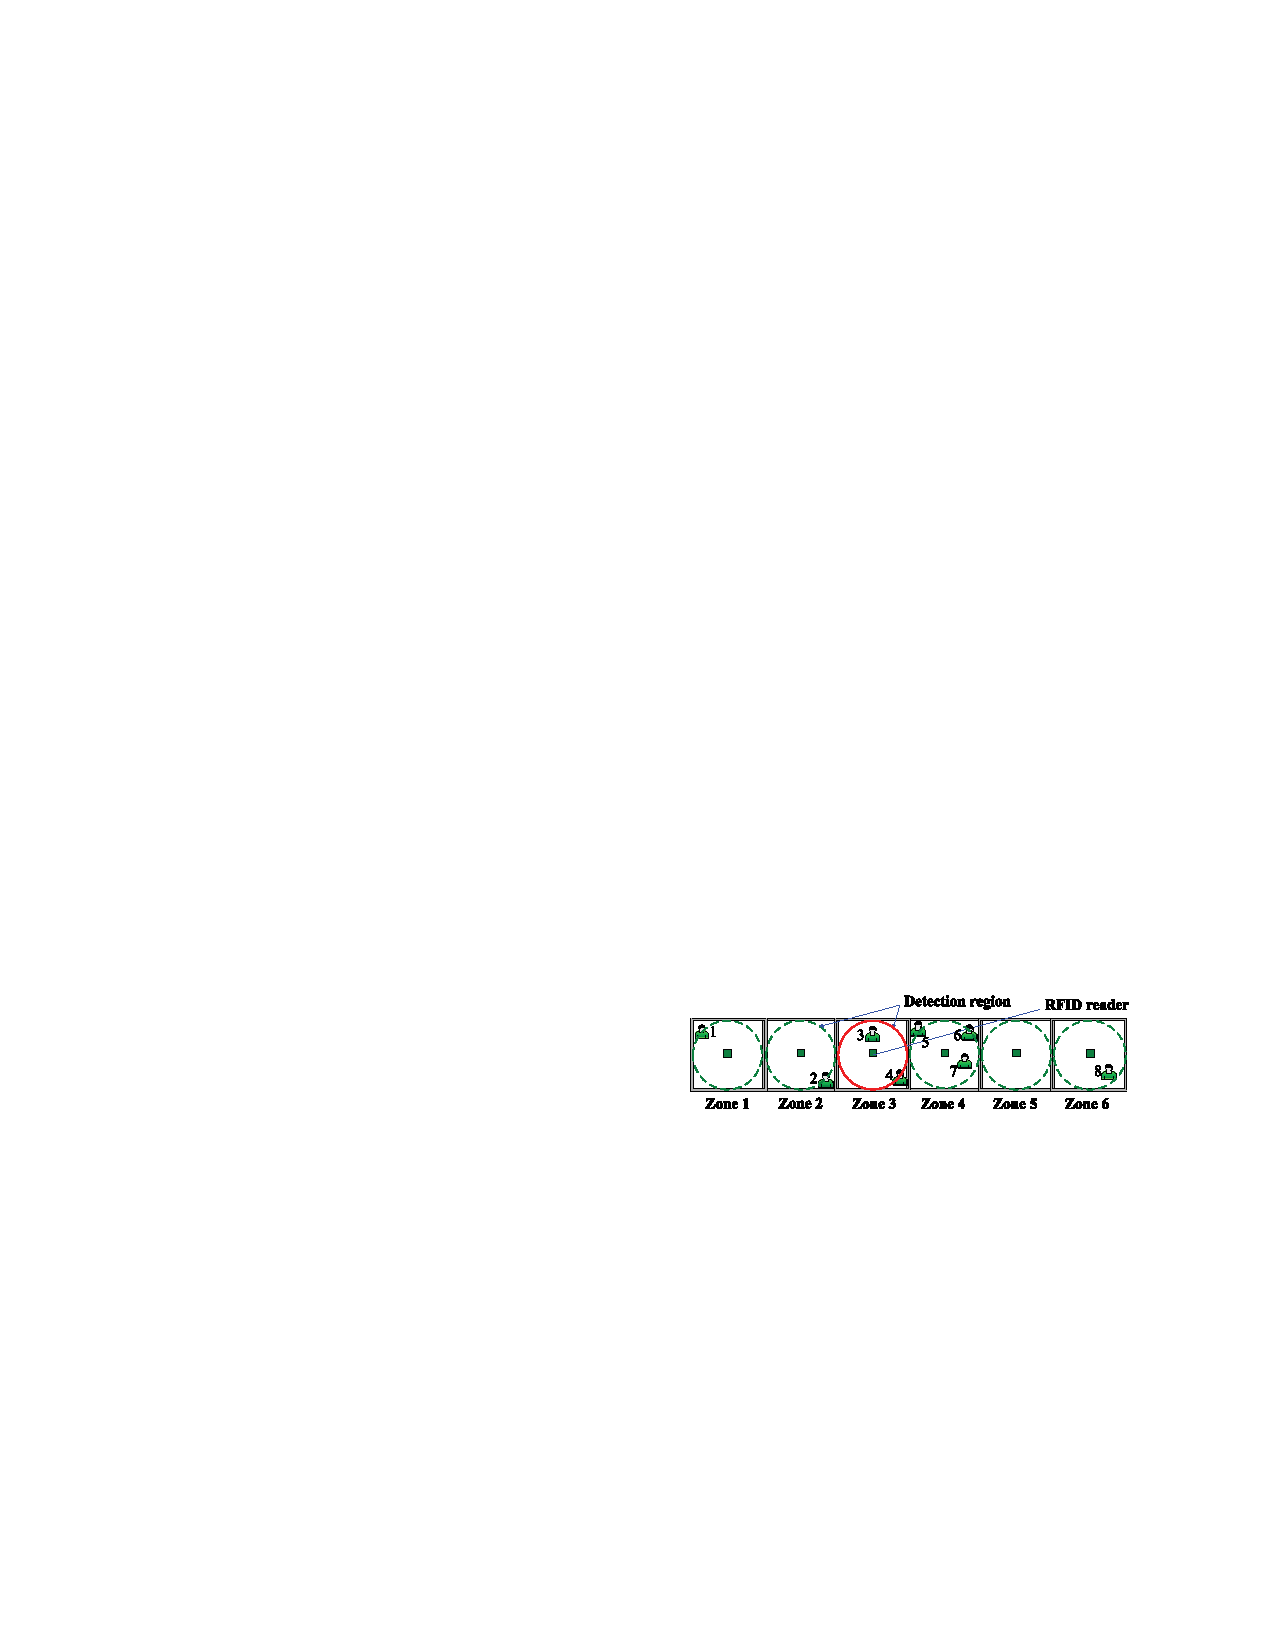
\includegraphics[width=0.8\columnwidth]{figures/3-1/3-1-4.pdf}
\end{figure}

A \conceptbf{simplified 2-state detection model} assumes readers' detection regions do not overlap, i.e., a reader is only able to detect the objects in its own zone. Then the likelihood can be estimated:

\begin{equation}
  p(z_{ij} = 1 | h_i) = \left\{\begin{matrix}
 r & \text{if}~h_i = j\\
 0 & \text{otherwise}
\end{matrix}\right.
\end{equation}

\begin{equation}
  p(z_{ij} = 0 | h_i) = \left\{\begin{matrix}
 1-r & \text{if}~h_i = j\\
 1 & \text{otherwise}
\end{matrix}\right.
\end{equation}

\end{frame}

%------------------------------------------------

\begin{frame}
\frametitle{RFID Reader Detection Model: The $n$-State}

The overall detection region of an RFID reader is divided into several sub-regions, each of which corresponds to a zone associated with a unique read rate.

\begin{figure}[tb]
  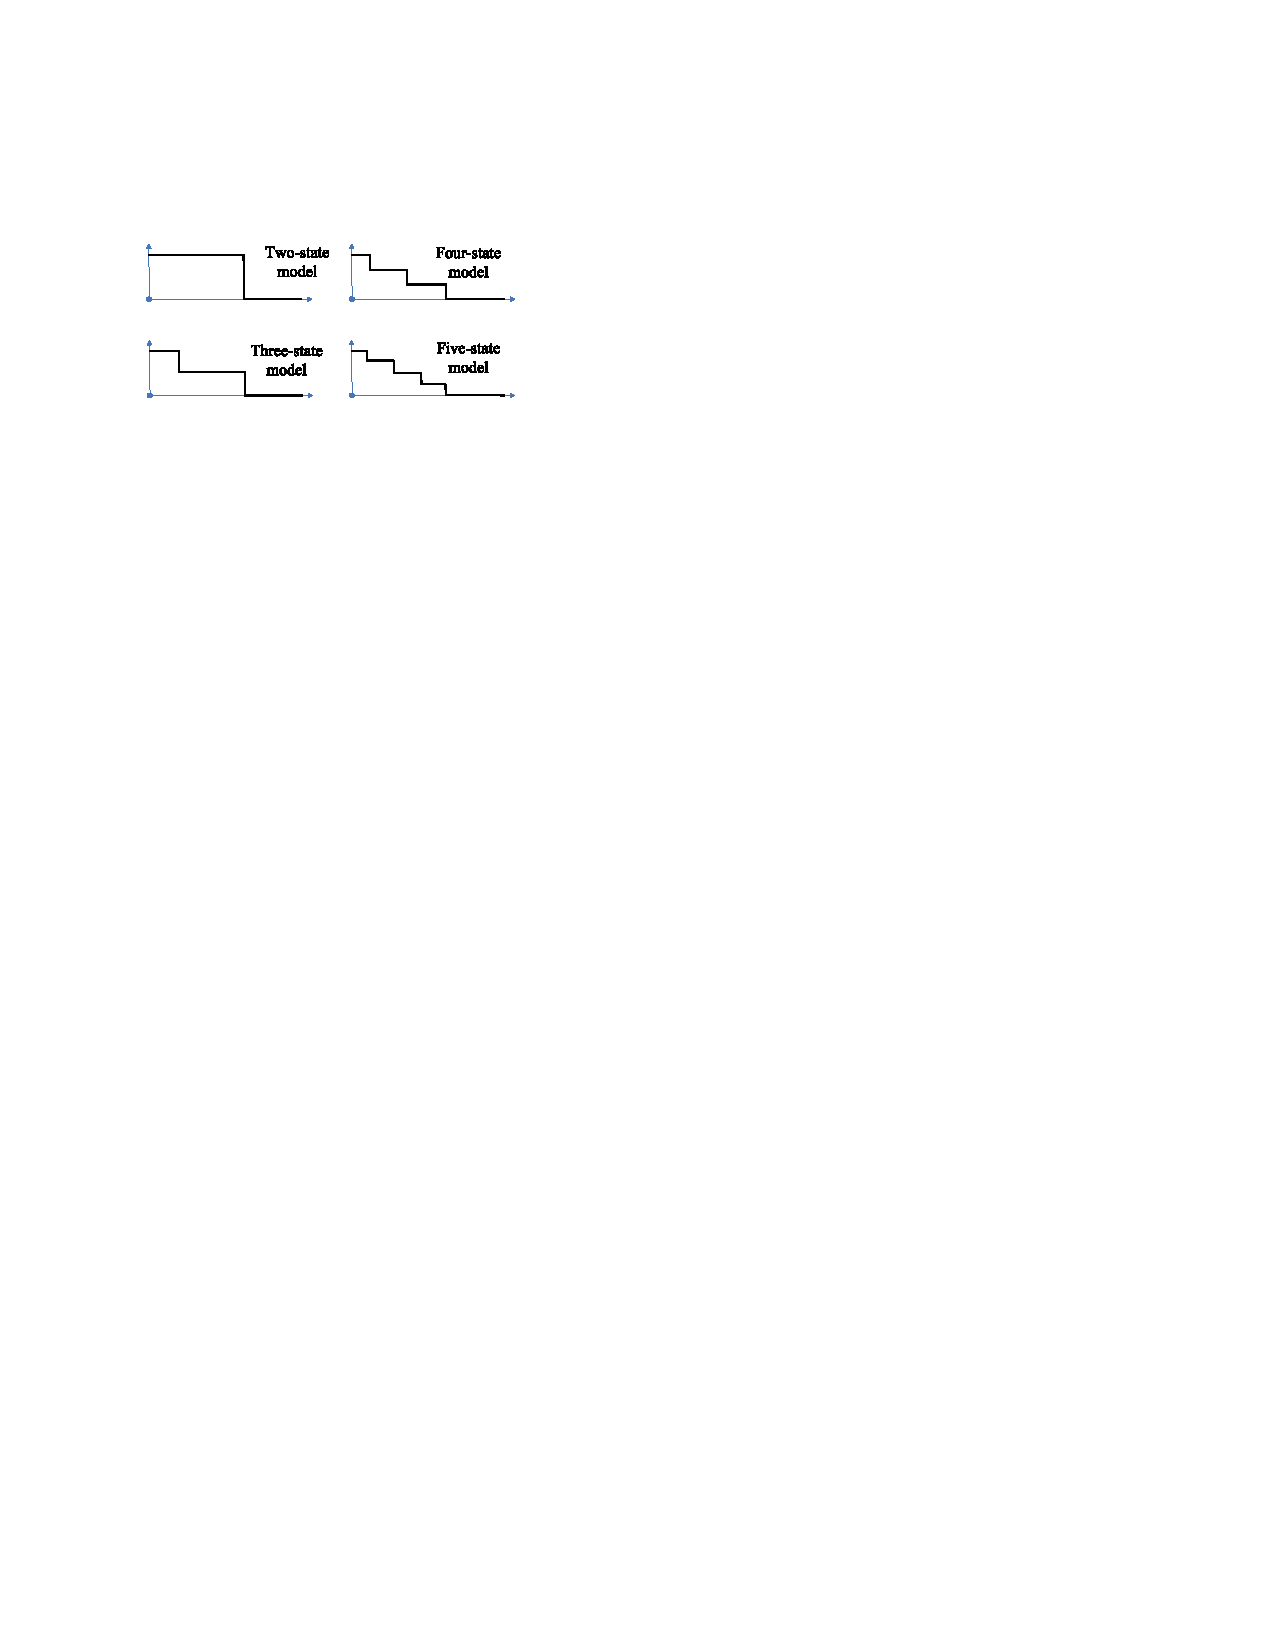
\includegraphics[width=0.8\columnwidth]{figures/3-1/3-1-5.pdf}
\end{figure}

Read rates for different states constitute an arithmetic sequence.

\end{frame}

%------------------------------------------------

\begin{frame}
\frametitle{A Case Study: The 3-State Model}

\begin{columns}[c]

  \column{0.4\textwidth}
  \begin{figure}[tb]
    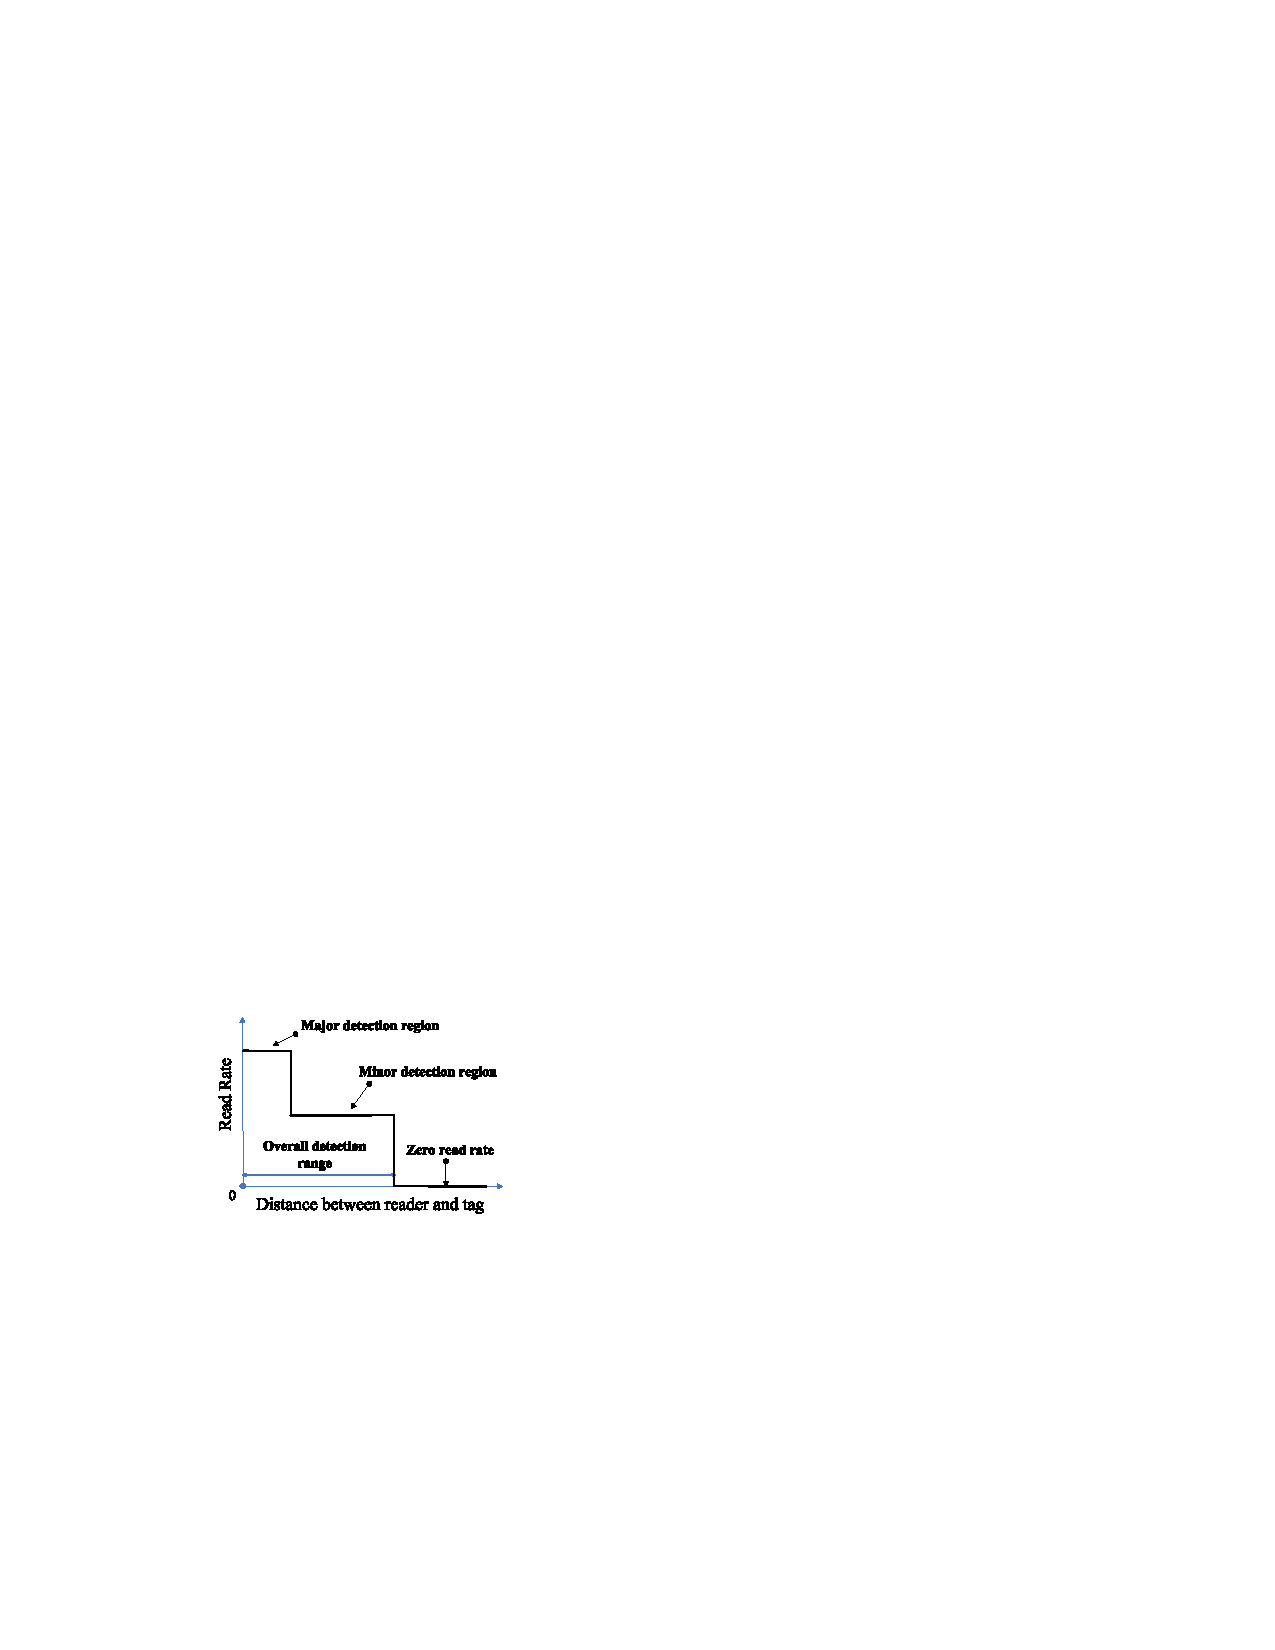
\includegraphics[width=\columnwidth]{figures/3-1/3-1-6.pdf}
  \end{figure}

  \column{0.6\textwidth}
  \begin{figure}[tb]
    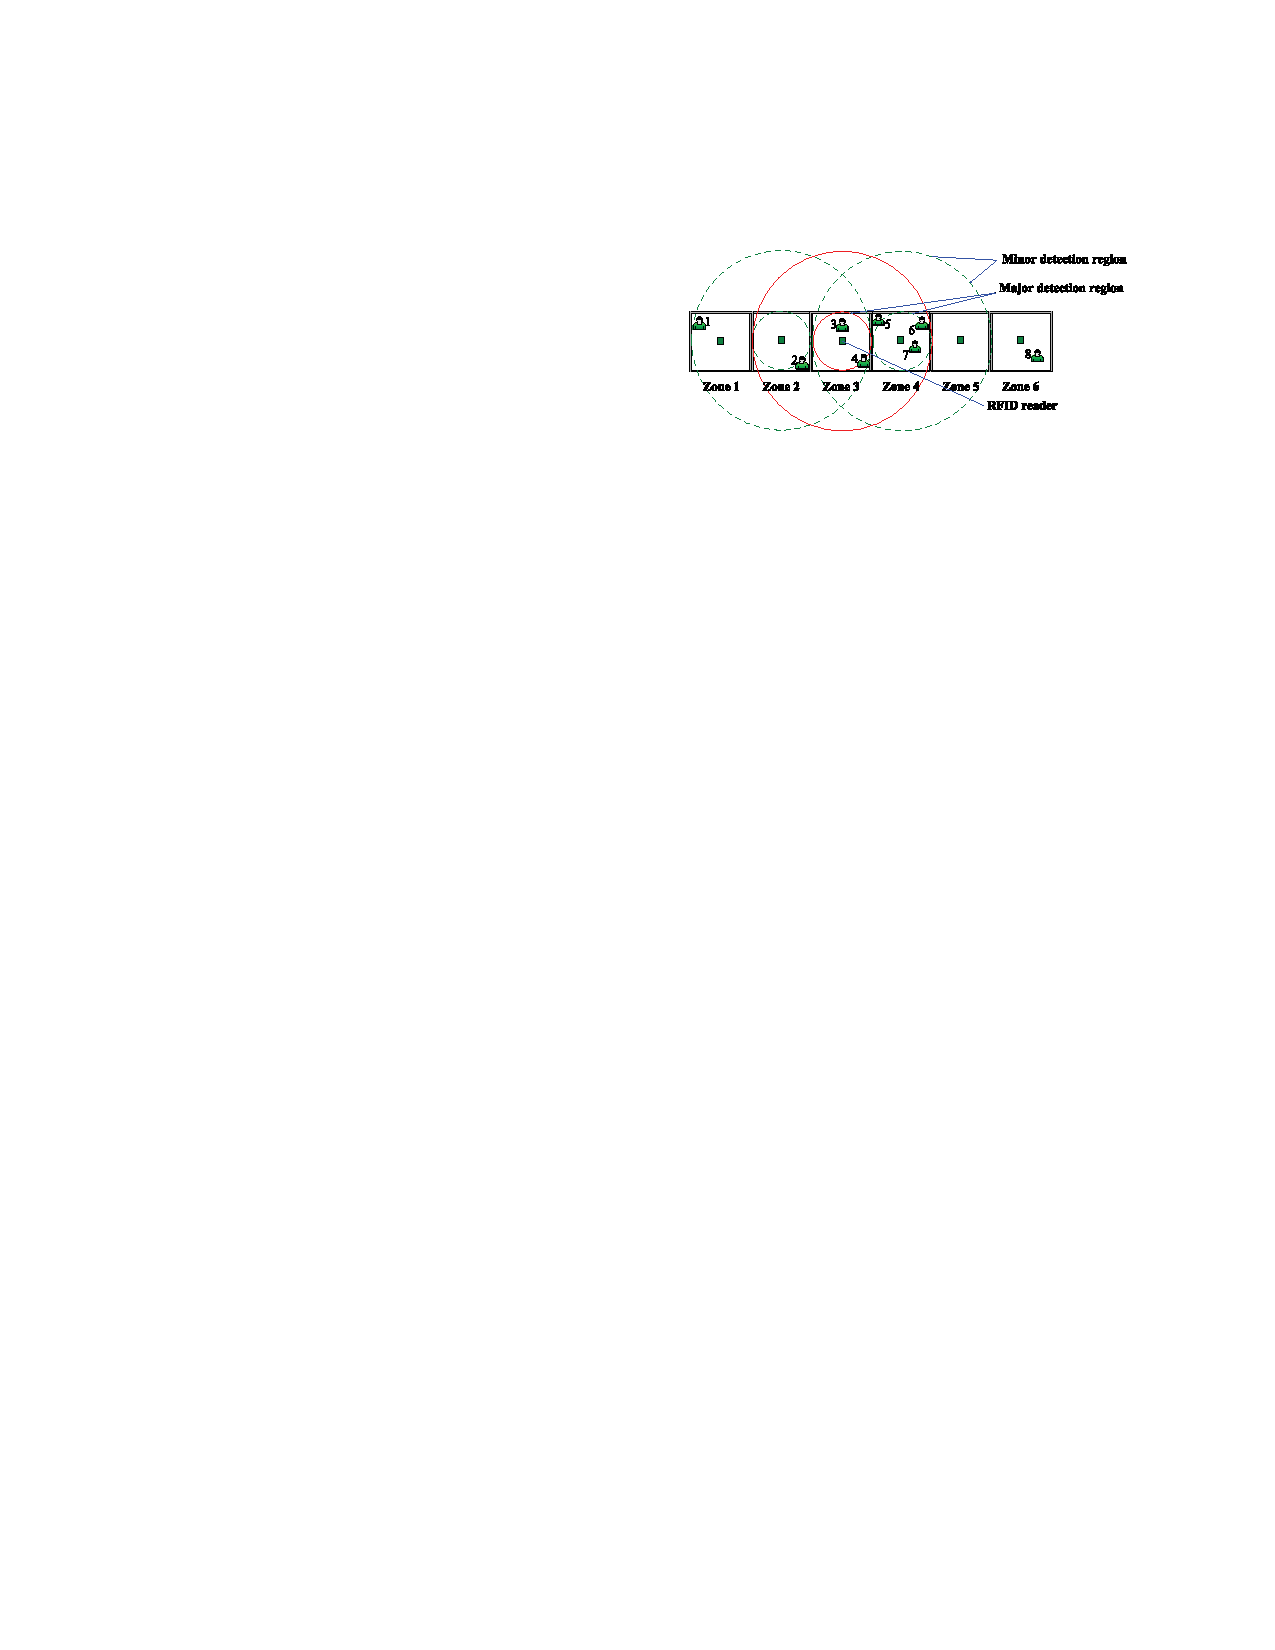
\includegraphics[width=\columnwidth]{figures/3-1/3-1-7.pdf}
  \end{figure}

\end{columns}

\vspace{10pt}
\begin{equation}
  p(z_{ij} = 1 | h_i) = \left\{\begin{matrix}
 r_{major} & \text{if}~h_i = j\\
 r_{minor} & \text{if}~h_i \in \{j-1, j+1\}\\
 0 & \text{otherwise}
\end{matrix}\right.
\end{equation}

\begin{equation}
  p(z_{ij} = 0 | h_i) = \left\{\begin{matrix}
  1- r_{major} & \text{if}~h_i = j\\
  1- r_{minor} & \text{if}~h_i \in \{j-1, j+1\}\\
 1 & \text{otherwise}
\end{matrix}\right.
\end{equation}

\end{frame}

%------------------------------------------------

\begin{frame}
\frametitle{Entropy Analysis}

\conceptbf{Entropy} can be used to measure the uncertainty in a system after invalid system states have been eliminated by a data cleansing method.\\~\\

Applying an efficient data cleansing method will lead to systems with smaller entropy.

\end{frame}

%------------------------------------------------

\begin{frame}
\frametitle{Entropy versus Read Rate}


\ssize{
  suppose that $y$ denotes the read rate in the 2-state detection model. The probabilistic mass function of $L$ in the 2-state model can be represented as:
  \begin{equation}
    p(L=l) = \left\{\begin{matrix}
    \alpha(1-y)y(1-y)\beta & \text{if}~l = j\\
    \alpha(1-y)(1-y)y\beta & \text{if}~l \in \{j-1,j+1\}\\
   0 & \text{otherwise}
  \end{matrix}\right.
  \end{equation}
  where $\alpha$ is the normalizing constant and $\beta$ represents the prior probability (assume that the prior distribution as a uniform distribution)
}

\begin{block}{Entropy of the 2-State model}
  \begin{equation}
    \begin{split}
      H(L) = & - \alpha(1-y)(1-y)y\beta \cdot ln(\alpha(1-y)(1-y)y\beta) \\
             & - \alpha(1-y)y(1-y)\beta \cdot ln(\alpha(1-y)y(1-y)\beta) \\
             & - \alpha(1-y)(1-y)y\beta \cdot ln(\alpha(1-y)(1-y)y\beta) \\
    \end{split}
  \end{equation}
  Because the probabilities on all the locations sum to 1, it has $\alpha\beta = \frac{1}{3(1-y)^2y}$. Therefore, it can be obtained: $  H(L) = -3 \cdot \frac{1}{3} \cdot ln\frac{1}{3} = 1.098 $
\end{block}
\end{frame}

%------------------------------------------------

\begin{frame}
\frametitle{Entropy versus Read Rate}


\ssize{
suppose $x$ is the read rate in the major detection
region. Then the read rate in the minor detection region can be
denoted as $x/2$. The probabilistic mass function of $L$ in the 3-state model can be represented as:
  \begin{equation}
    p(L=l) = \left\{\begin{matrix}
    \alpha(1-\frac{x}{2})x(1-\frac{x}{2})\beta & \text{if}~l = j\\
    \alpha(1-\frac{x}{2})(1-x)\frac{x}{2}\beta & \text{if}~l \in \{j-1,j+1\}\\
   0 & \text{otherwise}
  \end{matrix}\right.
  \end{equation}
}

\vspace{-10pt}
\begin{block}{Entropy of the 3-State model}
  \begin{equation}
    \begin{split}
      H(L) = & - \alpha(1-\frac{x}{2})(1-x)\frac{x}{2}\beta \cdot ln(\alpha(1-\frac{x}{2})(1-x)\frac{x}{2}\beta) \\
             & - \alpha(1-\frac{x}{2})^2x\beta \cdot ln(\alpha(1-\frac{x}{2})^2x\beta \\
             & - \alpha(1-\frac{x}{2})(1-x)\frac{x}{2}\beta \cdot ln(\alpha(1-\frac{x}{2})(1-x)\frac{x}{2}\beta) \\
    \end{split}
  \end{equation}
  Since probabilities on all locations sum to 1, it has $\alpha\beta = \frac{1}{x(1-\frac{x}{2})(2-\frac{3x}{2})}$, and $  H(L) = -2 \cdot \frac{1-x}{4-3x} \cdot ln\frac{1-x}{4-3x} - \frac{2-x}{4-3x} \cdot ln\frac{2-x}{4-3x} $
\end{block}
\end{frame}

%------------------------------------------------

\begin{frame}
\frametitle{Variations on Entropy}

\begin{columns}[c]

\column{0.47\textwidth}
\begin{figure}[tb]
  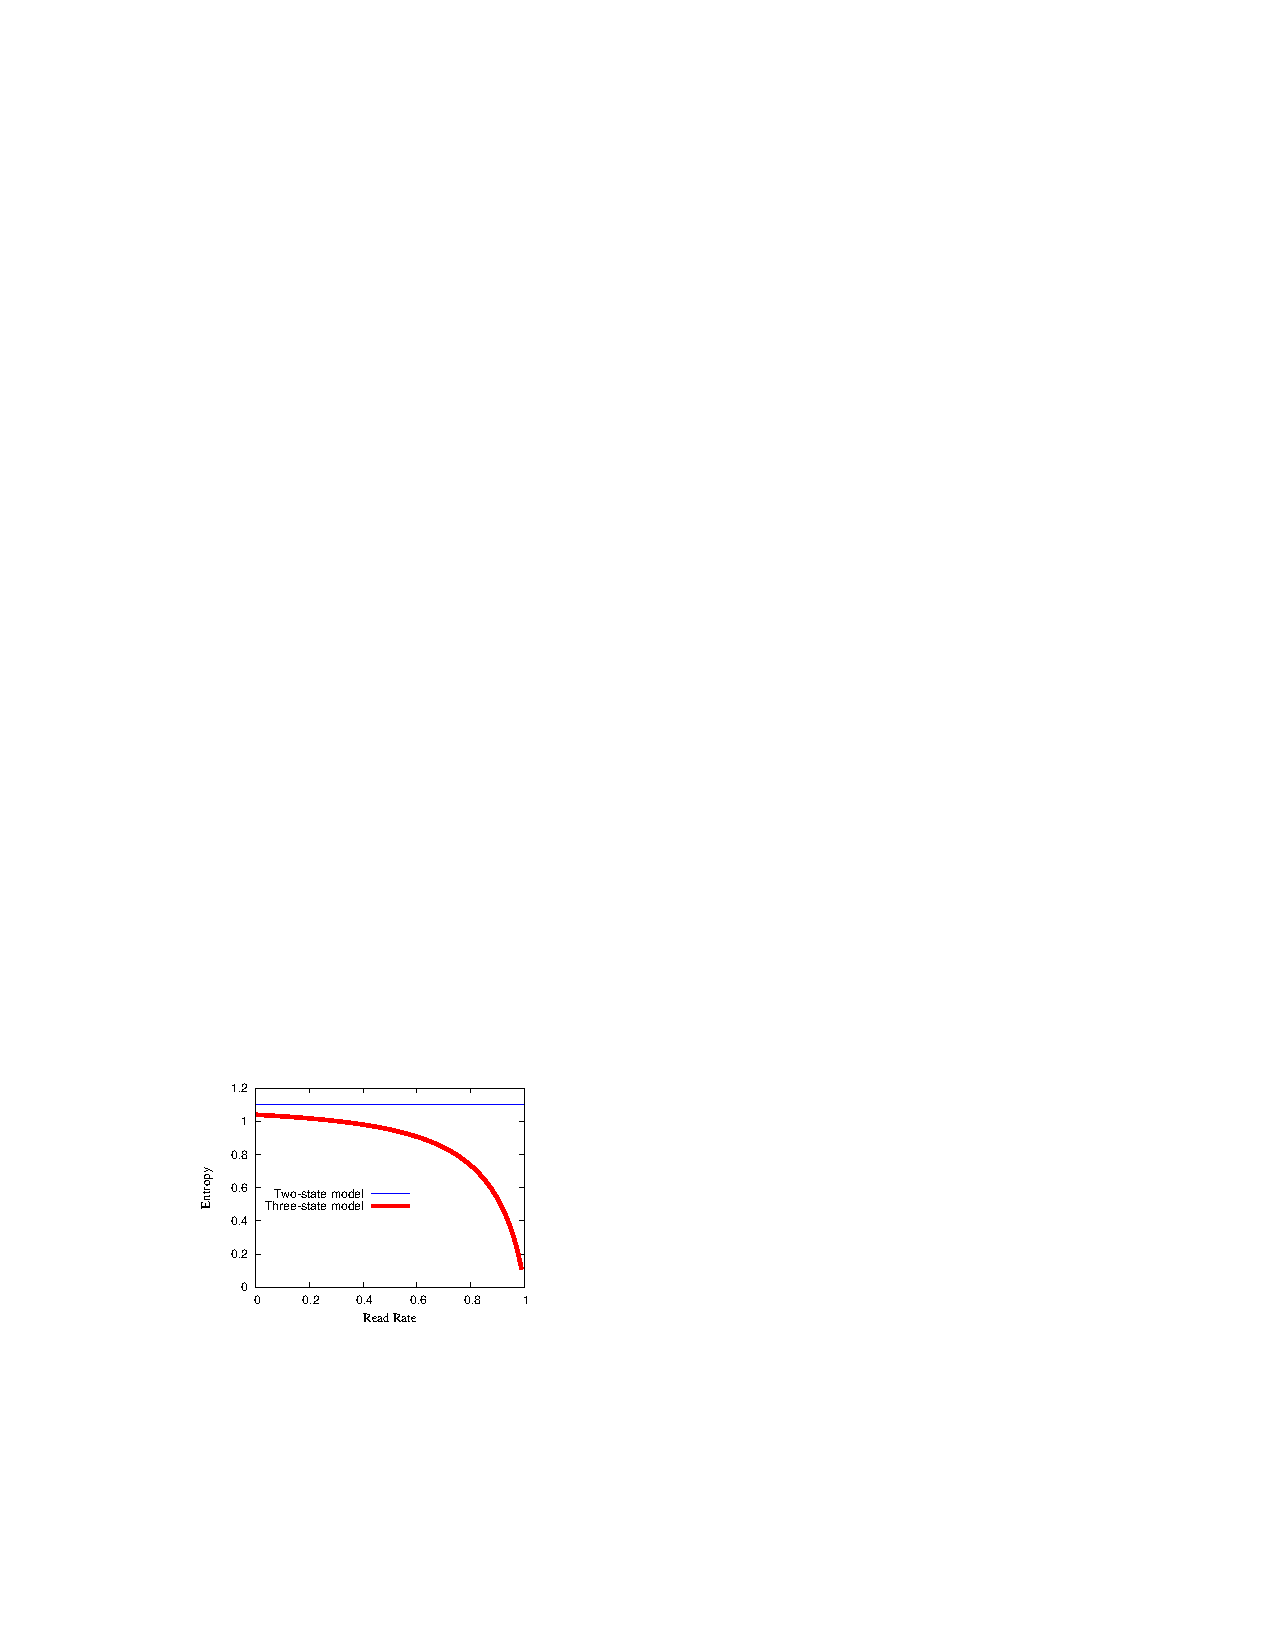
\includegraphics[width=\columnwidth]{figures/3-1/3-1-8.pdf}
  \caption{\ssize{Relationship between entropy and read rate in the 2-state and 3-state models for read rate $x=0.95$.}}
\end{figure}

\column{0.53\textwidth}
\begin{figure}[tb]
  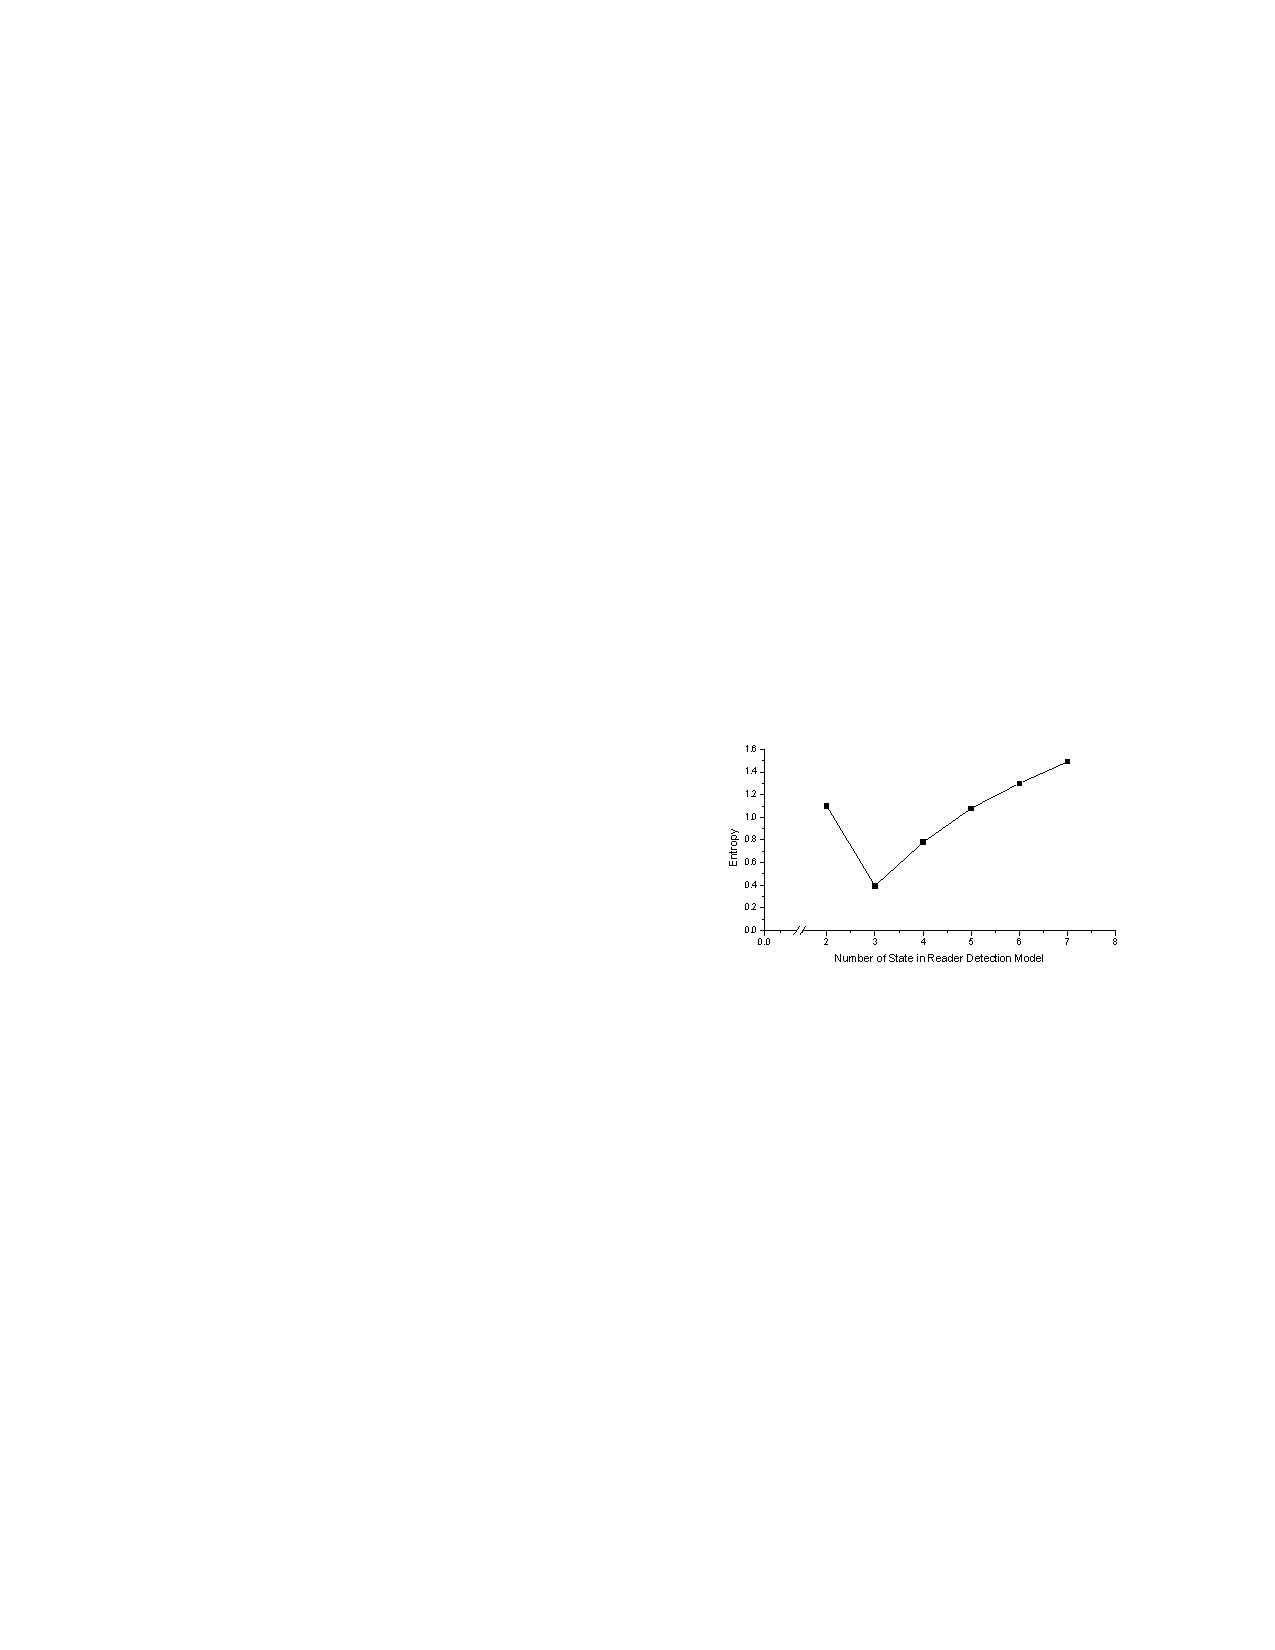
\includegraphics[width=\columnwidth]{figures/3-1/3-1-9.pdf}
  \caption{\ssize{Relationship between entropy and the number of states in a detection model.}}
\end{figure}

\end{columns}

\end{frame}

%------------------------------------------------

\begin{frame}
\frametitle{Markov Chain Monte Carlo}

\conceptbf{Markov Chain Monte Carlo (MCMC)}\cite{andrieu2003introduction} is a technique to generate samples from the state space by simulating a Markov chain.\\~\\

The formed Markov chain is constructed in such a way that the chain spends more time in the regions with higher importance (i.e., the Markov chain converges to the posterior as its stationary distribution).

\end{frame}

%------------------------------------------------

\begin{frame}
\frametitle{Metropolis-Hastings Sampling}

\begin{columns}[c]

\column{0.5\textwidth}
\begin{figure}[tb]
  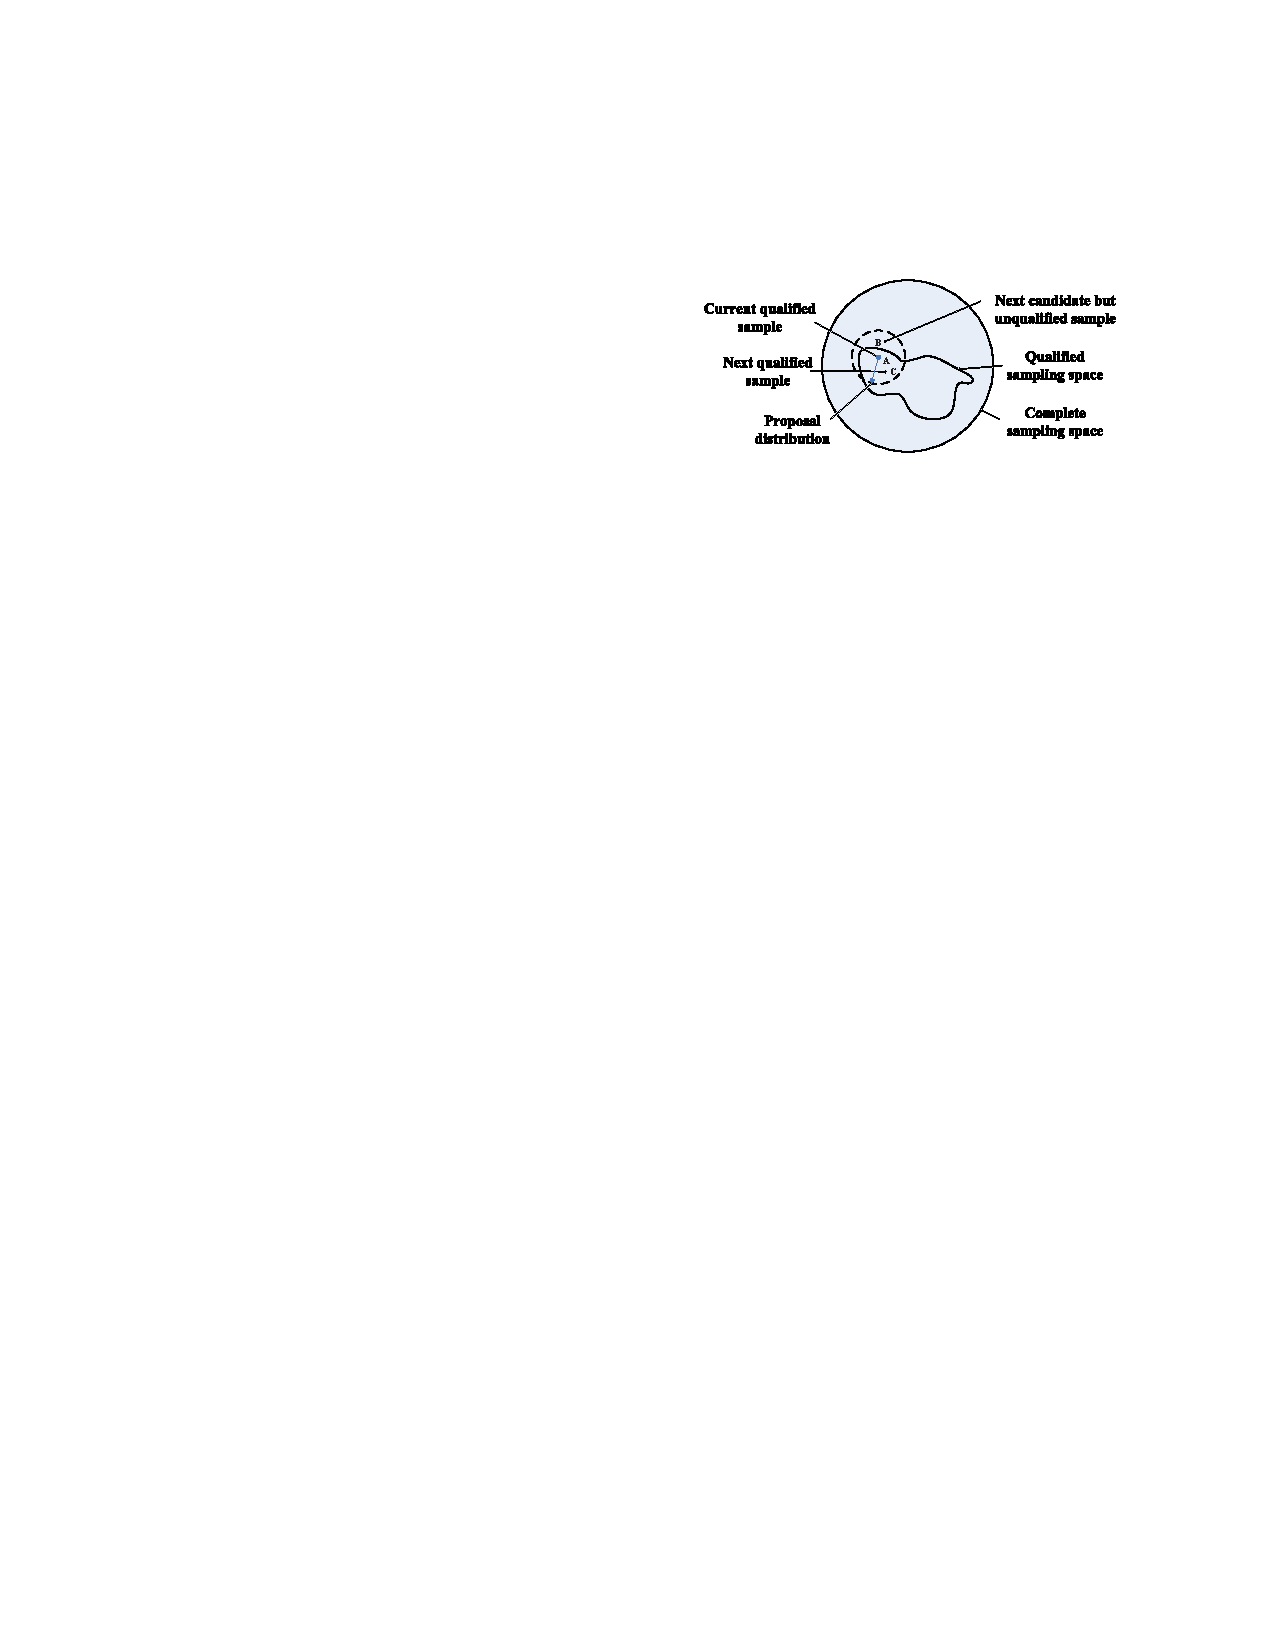
\includegraphics[width=\columnwidth]{figures/3-1/3-1-10.pdf}
\end{figure}

\column{0.5\textwidth}
\begin{example}
  \ssize{
  If a MCMC-based sampler is employed, the next sample will be chosen according to proposal distribution at point A, thus the probability that the next sample generated by MCMC falls into the qualified sampling space is considerably increased.
  }
\end{example}

\end{columns}

\begin{block}{Metropolis-Hastings Algorithm}
Suppose $\hat{H_{t-1}}$ is the immediate previous state before the state $\hat{H_t}$ in the formed Markov chain. According to \conceptbf{Metropolis-Hastings} algorithm, at fist, a proposal sample $\hat{H_q}$ is drawn from a proposal distribution $q(\hat{H_q}|\hat{H_{t-1}})$. Then \emph{Metropolis-Hastings} accepts $H'$ as the next state $\hat{H_t}$ with the probability of $\frac{post(H'|\mathbb{Z})}{post(H_{t-1}|\mathbb{Z})}$.
\end{block}


\end{frame}

%------------------------------------------------

\begin{frame}
\frametitle{Metropolis-Hastings Sampling With Constraints}

\conceptbf{Metropolis-Hastings Sampling With Constraints (MH-C)}: To incorporate constraints in sampling in order to reject some inapplicable(not qualified) samples.\\~\\

Each zone is associated with multiple variables call \emph{resource descriptors}, representing how much the ssociated resource is still available. The variable is denoted as $Des_{zone_i}$, check if an object with volume $Vol_{object_j}$ is able to be store by:
\begin{equation}
  Des_{zone_i} = Des_{zone_i} - Vol_{object_j}
\end{equation}

The proposed resource allocation is feasible only if $Des_{zone_i}$ is no less than zero, otherwise a re-sampling is required.

\end{frame}

%------------------------------------------------

\begin{frame}
\frametitle{MH-C Algorithm}

Symbol notations used in MH-C algorithm:

\begin{figure}[tb]
  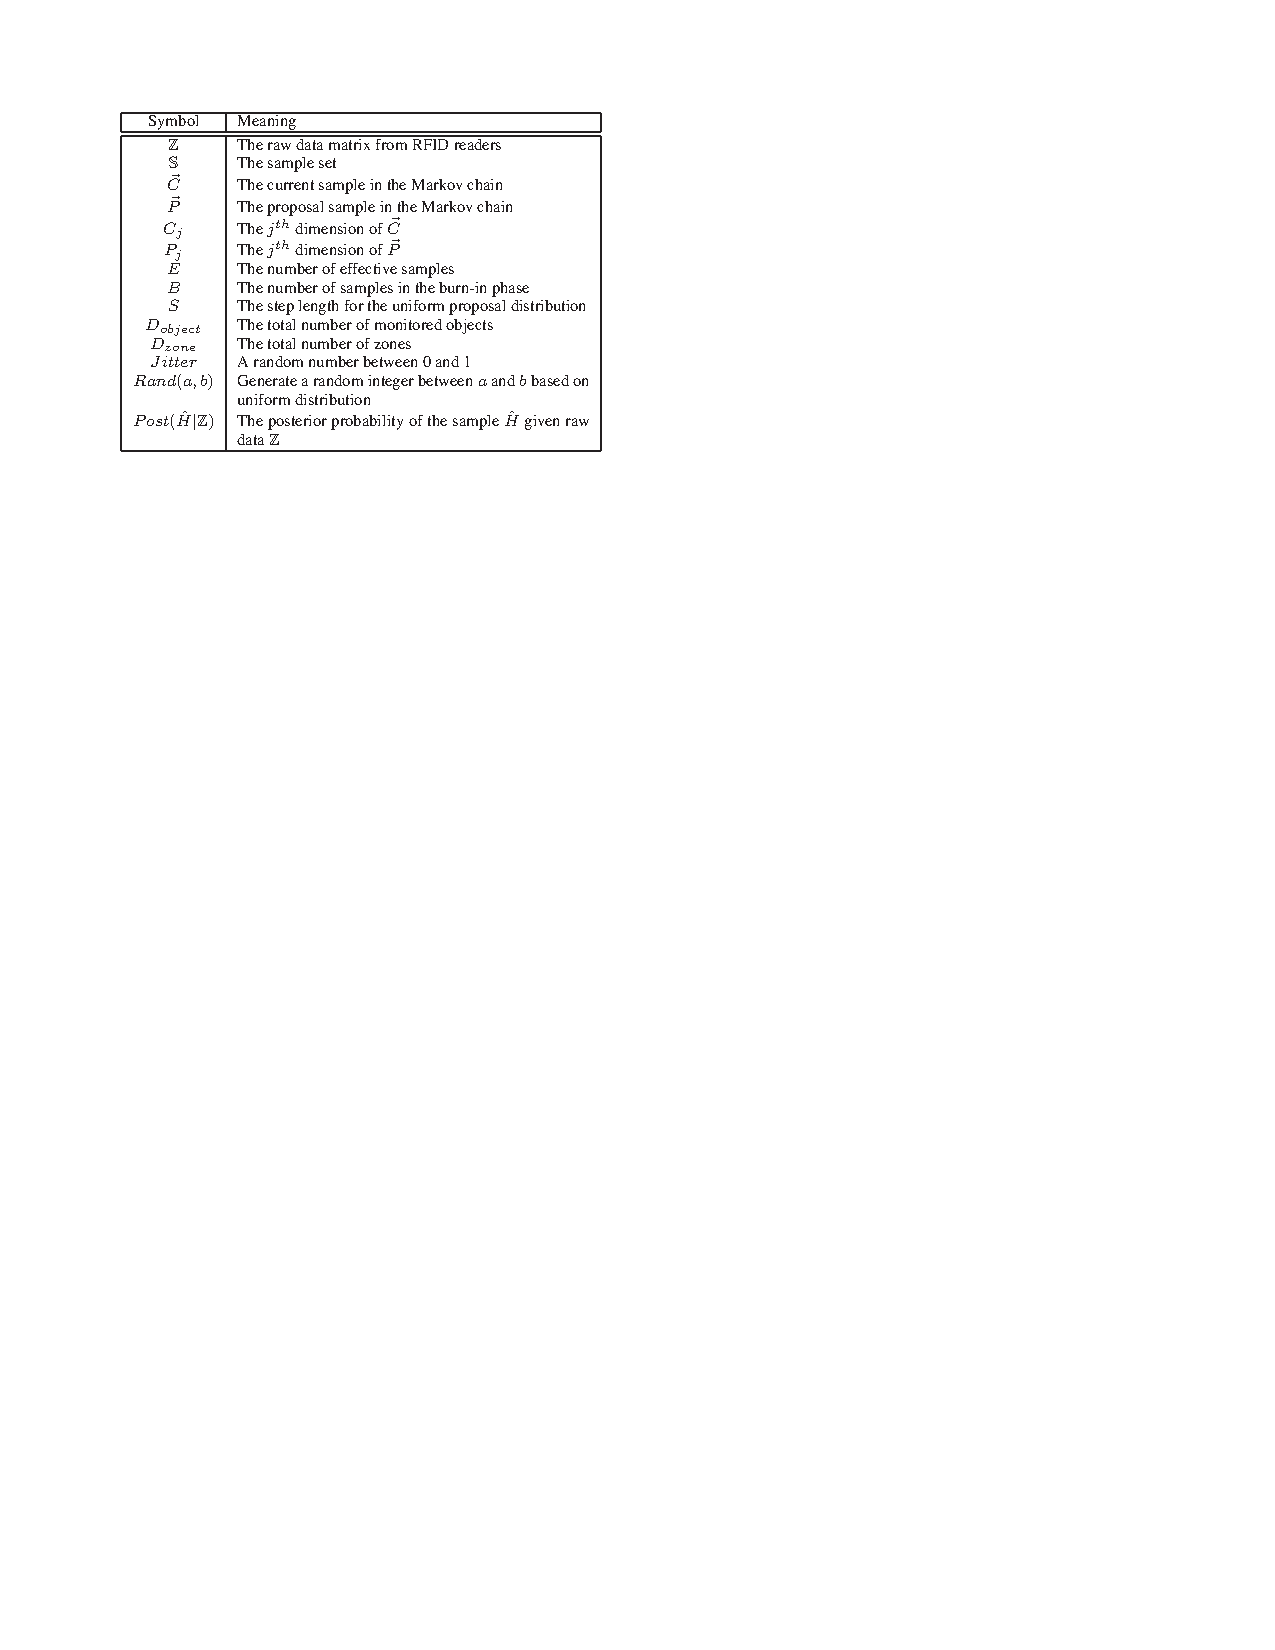
\includegraphics[width=0.7\columnwidth]{figures/3-1/3-1-11.pdf}
\end{figure}

\end{frame}

%------------------------------------------------

\begin{frame}
\frametitle{MH-C Algorithm}

\begin{columns}[c]

\column{0.45\textwidth}
\begin{figure}[tb]
  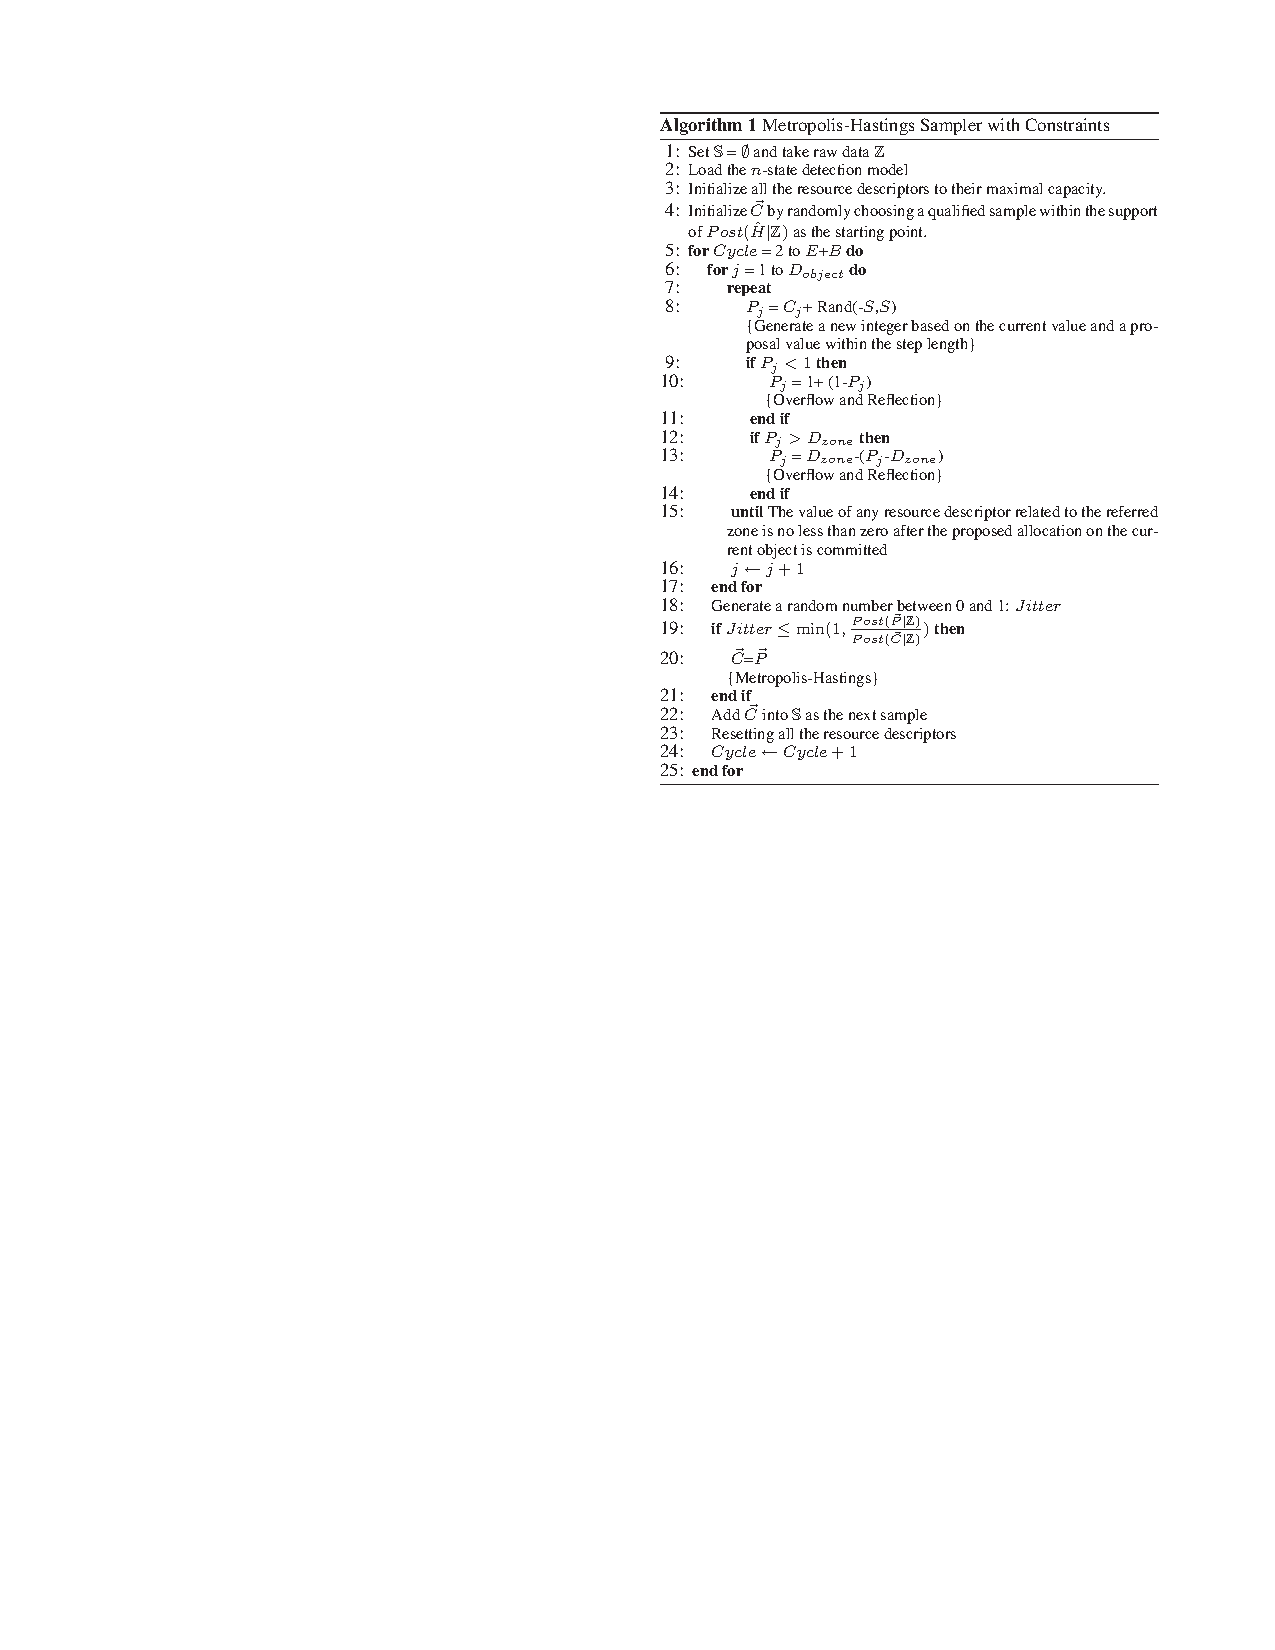
\includegraphics[width=\columnwidth]{figures/3-1/3-1-12.pdf}
\end{figure}

\column{0.55\textwidth}
\begin{sitemize}
  \item Line 1: initializes the sample set and takes the RFID raw data;
  \item Line 2: loads the $n$-state detection model of readers with the objective of computing the likelihood;
  \item Line 3--4: initializes all the resource descriptors and randomly chooses a qualified sample as the first state of the Markov Chain;
  \item Lines 6--17: generate a random sample as the proposal sample dimension by dimension (object by object);
  \item Lines 18--21: accept the proposal sample as the next state of Markov chain with the probability of the posterior ratio of the proposal sample over the current sample;
  \item Lines 22--23: add the next state into the sample set and reset the zone resources.
\end{sitemize}

\end{columns}

\end{frame}

%------------------------------------------------

\begin{frame}
\frametitle{Available Queries}

With a large mount of qualified samples, the approach enables two important types of queries against RFID raw data: \\~\\

Given an object and a zone, a \conceptbf{Location Query} returns the probability that the object is in that zone.\\~\\

Given a zone, a \conceptbf{Remaining Capacity Query} returns the leftover volume of a certain resource available in that zone.\\~\\

\end{frame}

%------------------------------------------------

\begin{frame}
\frametitle{Conclusions}

\ssize{
The data reported by RFID devices are known to be unreliable.\\~\\

This work proposed a Bayesian inference based approach for cleansing RFID rww data which can take advantage of duplicate readings.\\~\\

In order to evaluate the location and aggregate queries, the approach employs prior knowledge to quantify the degree of uncertainty on the location of each object and remaining capacity in each zone.\\~\\

$n$-State detection model is proposed to capture likelihood and validate that the 3-state model can maximize the system performance.\\~\\

MH-C was devised to efficiently sample from the posterior distribution environmental constraints.
}

\end{frame}
